\documentclass[10pt,xcolor={x11names}]{beamer}
\usetheme{Warsaw}
\usepackage{tikz}
\usepackage{pgf-pie}
\usepackage{pgfplots}
\usepackage{xcolor}
\newcommand\tab[1][1cm]{\hspace*{#1}}
\usepackage{fancyvrb}
\usepackage{xspace}
\usepackage[utf8]{inputenc}
\usepackage{graphicx}



\newcommand{\themename}{\textbf{\textsc{metropolis}}\xspace}

\makeatletter
\newcommand\titlegraphicii[1]{\def\inserttitlegraphicii{#1}}
\titlegraphicii{}
\setbeamertemplate{Presentaciòn Beamer}
{
  \vbox{}
   {\usebeamercolor[fg]{titlegraphic}\inserttitlegraphic\hfill\inserttitlegraphicii\par}
  \begin{centering}
    \begin{beamercolorbox}[sep=8pt,center]{institute}
      \usebeamerfont{institute}\insertinstitute
    \end{beamercolorbox}
    \begin{beamercolorbox}[sep=8pt,center]{title}
      \usebeamerfont{title}\inserttitle\par%
      \ifx\insertsubtitle\@empty%
      \else%
        \vskip0.25em%
        {\usebeamerfont{subtitle}\usebeamercolor[fg]{subtitle}\insertsubtitle\par}%
      \fi%     
    \end{beamercolorbox}%
    \vskip1em\par
    \begin{beamercolorbox}[sep=8pt,center]{date}
      \usebeamerfont{date}\insertdate
    \end{beamercolorbox}%\vskip0.5em
    \begin{beamercolorbox}[sep=8pt,center]{author}
      \usebeamerfont{author}\insertauthor
    \end{beamercolorbox}
  \end{centering}
  %\vfill
}
\makeatother
\title{Presentacion Beamer}
\subtitle{Proyecto 1}
\institute{Compiladores e Interpretes \\ Instituto Tecnologico de Costa Rica}
\date{2020}

\begin{document}

\begin{frame}[plain]
\maketitle
\small
Profesor: Dr. Jose Francisco Torres\par\medskip
\begin{tabular}[t]{@{}l@{\hspace{3pt}}p{.32\textwidth}@{}}
Examiners:  \\
& Nakisha Dixon 2017103353 \\
& Andrei Leon 201015265 \\
& Francisco Pereira 2017238806
\end{tabular}%
\footnotesize
\end{frame}

\begin{frame}{Table of contents}
  \setbeamertemplate{section in toc}[sections numbered]
  \tableofcontents[hideallsubsections]
\end{frame}



\section{Introduccion}

\begin{frame}[fragile,allowframebreaks]{Flex}
        \begin{alertblock}{Scanner}
            FLEX (generador de analizador léxico rápido) es una herramienta para generar analizadores léxicos (escáneres o lexers) escrito por Vern Paxson en C alrededor de 1987. Se usa junto con el generador de parser Berkeley Yacc o el generador de parser GNU Bison
            \end{alertblock}
\end{frame}

\begin{frame}
\frametitle{Proceso de Scanning}
\begin{itemize}
 \item<1-> Flex genera un archivo .C como salida, ‘lex.yy.c’ (contiene un montón de código incomprensible pero que básicamente contiene las reglas que especificamos en el incluyendo el código para las acciones que especifiquemos). Este archivo contiene una extern function llamada yylex() que escanea un token. 
 \item<2-> Este archivo se compila y se conecta con la librería ‘lfl’ para producir un ejecutable. Cuando se corre el ejecutable, analiza cierta entrada buscando ocurrencias de las expresiones regulares. 
 \item<3> Cuando encuentra cierta expresión regular, ejecuta cierto código correspondiente que se le asignó. 
\end{itemize}
\end{frame}

\section{Analisis Léxico}

\begin{frame}[fragile,allowframebreaks]{Analisis Léxico}
        \begin{alertblock}{Codigo fuente}
            A continuación se presenta el código fuente con colores demostrando la división de \textit{tokens}.
            \end{alertblock}
        
\end{frame}

\begin{frame}[fragile,allowframebreaks]{Analisis Léxico|claves de color}
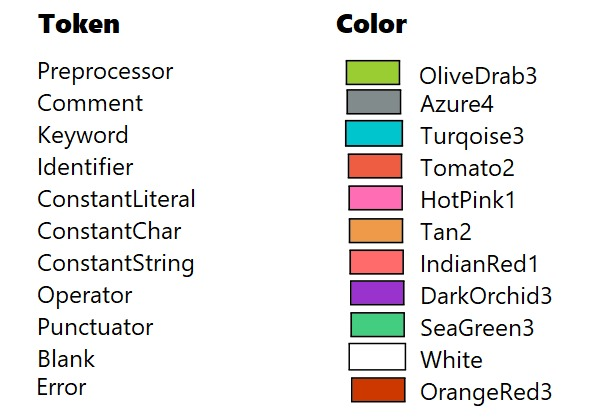
\includegraphics[width=8cm]{colors}
\end{frame}

\begin{frame}[fragile,allowframebreaks]{Syntax Highlighting}~\color{Rhodamine}\begin{verbatim}/* Hello
   sdfsdf
   World program */\end{verbatim}\leavevmode\newline\newline\color{Gray}\verb$#include <stdio.h>$\newline\color{Rhodamine}\begin{verbatim}/* here another comment */\end{verbatim}\leavevmode\newline\color{Aquamarine}\verb$main$\color{Fuchsia}\verb$($\color{Fuchsia}\verb$)$\newline\color{Fuchsia}\verb${$\newline\tab\color{Aquamarine}\verb$printf$\color{Fuchsia}\verb$($\color{Emerald}\verb$"Hellow World"$\color{Fuchsia}\verb$)$\color{Fuchsia}\verb$;$\newline\tab\color{Aquamarine}\verb$printf$\color{Fuchsia}\verb$($\color{Emerald}\verb$"Hello World"$\color{Fuchsia}\verb$)$\color{Fuchsia}\verb$;$\newline\color{Fuchsia}\verb$}$\newline
\end{frame}


\section{Histograma}
\begin{frame}[fragile,allowframebreaks]{Histograma}
        \begin{alertblock}{Histograma}
            A continuación se presenta un histograma que muestra la cantidad de cada tipo de \textit{token} encontrado en el código fuente:
            \end{alertblock}
\end{frame}
\begin{tikzpicture}
  \begin{axis}[
	x tick label style={
		/pgf/number format/1000 sep=},
	ylabel=Cantidad de Tokens,
	enlargelimits=0.05,
	legend style={at={(0.5,-0.1)},
	anchor=north,legend columns=-1},
	ybar interval=0.7,
	nodes near coords,  x tick label style={rotate=45,anchor=east},
	symbolic x coords={PREPROCESSOR,COMMENT, KEYWORD, IDENTIFIER, CONSTANTLITERAL, CONSTANTCHAR, CONSTANTSTRING, OPERATOR, PUNCTUATOR, BLANK},
    ]
    
    \addplot
    table[x=x, col sep=comma,]
          {datafile.dat};
  \end{axis}
\end{tikzpicture}



\section{Conclusion}
\begin{frame}[fragile,allowframebreaks]{Grafico Pie}
        \begin{alertblock}{Pie Chart}
            A continuación se presenta un grafico de pie que muestra la cantidad de cada tipo de \textit{token} encontrado en el código fuente:
            \end{alertblock}
\end{frame}

\end{document}